\section{Smart Homes}
Another trend that utilizes the concept of IoT is smart homes which are homes that are, 
to some degree, automated by utilization IoT devices. 
The devices used for smart homes differ greatly from wearables as they are usually stationary. 
The concept of smart homes have been around for a while and numerous homes have already integrated some of these smart devices. 
A good example of a high-end smart home is Bill Gate's mansion in Medina, Washington \cite{billgatehouse}.
This \$100 million house have sensors to adjust each room's temperature and lighting, 
and have speakers behind the wallpaper that follows you from room to room. 
The artwork in the house is mostly digital and can be changed by pressing a button. 
One can only imagine what other technology is being used in that house. 

However, that is a rather extreme example of a smart home. 
Ordinarily, the devices found in smart homes are common items that has been connected to the Internet for wireless control.
Common devices that are found in smart homes include, but are not limited to, 
coffee machines, washers and dryers, thermostats, sound systems and locks. 
However, only few devices have really gained ground for the common user and few homes are automated.
One of the most commonly found IoT in homes are the Nest thermostat \cite{NEST}. 
This thermostat senses when you are around and when you are not to control the climate inside to save energy and thus money.
Unlike a lot of smart devices that are made to make your life a little easier, such as an automated coffee machine, 
the Nest thermostat helps you save money which is likely the reason for it popularity. 
Furthermore, the newest version (as of October 2015) allows you to connect other IoT devices to the thermostat. 
The Nest thermostat is thus starting to solve what is probable the greatest problem with smart homes (and IoT in general), 
and why they have not become popular yet: Lack of interconnectivity between IoT devices. 
This problem leads us to what is known as smart hubs. 

\subsection{Smart Hubs}
A smart hub is a device, or service, that implements several communication protocols used by IoT devices, 
and gives the user a single protocol or interface. 
The goal of a smart hub is to make the connected devices able to communicate. 

\subsubsection{Common Protocols for IoT}
There is a range of different protocols that are being used for various smart devices. 
We will not get into much detail with these protocols, 
but we demonstrate how many different there are and why communication is a problem.
\begin{table}
   \begin{description}
       \item[Protocol:] ZigBee
       \item[Used by:] Samsung, Jasco, Smartenit, FortrezZ and others
       \item[In products:] SmartThings Hub, thermostats, door sensors, light bulbs, etc.\\
       
       \item[Protocol:] Z-Wave
       \item[Used by:] FortrezZ, GE, Intermatic, Leviton, Aeon Labs, Evolve and others
       \item[In products:] Thermostats, wall outlets, door locks, door and window sensors, etc.  \\
       
       \item[Protocol:] WiFi (IEEE 802.11)
       \item[Used by:] Nest, Philips, Samsung, Bose, D-link and others
       \item[In products:] Thermostats, speakers, light bulbs, motion sensors, fitness trackers, camera, etc. 
    \end{description}
    \caption{Protocols used by various IoT devices}\label{table:iotprotocols}
\end{table}

Aside from the protocols in \Cref{table:iotprotocols}, 
there are several others messaging protocols such as MQTT, CoAP and XMPP used by various devices. 

A smart hub should thus not only be able to communicate with the devices, 
but also be able to transform the data to a single format and give easy access to it. 

\subsubsection{Smart Hubs on the Market}
The requirements for smart hubs have gained the attention of several large companies and even more smaller companies, 
all competing to be center of future smart homes. 
%Something about SmartThings
%How does wearables fit in

\subsection{Indoor Positioning}\label{sec:indoor-positioning}
%Something about Estimote
In order to determine which device the user points at and thereby intends to control, 
it is necessary to determine the locations of the devices in the system relative to the user.

The focus of this project is not to position devices and as such it was not the intention to spend time developing an entire solution for positioning devices indoors. 
Instead it was desired to find an existing product that could be used to facilitate indoor positioning.
The solution should be available in the early phases of the project in order to start building the system based on the solution for positioning.

Ideally users of this project should be able to control any device that fits within the concept of Internet of Things he owns, 
the price for any device needed to position each controllable device should be low. 
If a user owns several devices that can be controlled using gestures and an extra device is needed for each in order to preform the positioning, 
the price of such a device should be at a minimum.

It is assumed that users already own one or more devices that fit within the concept of Internet of Things and possibly are early adapters of such technology, 
it is assumed they have some technological expertise. 
However, it easy to imagine that this project can be used in an office environment where employees of varying technological expertise work or in health care. 
Therefore users may have a varying degree of technological expertise and it should be easy to extend the solution with new controllable devices.

Naturally the accuracy of the solution used for positioning objects plays an important part. 
\Cref{fig:indoor-positioning:incorrect} shows the consequence of an incorrect location. 
If a lamp is estimated to be at another location that it is actually located, 
the user must point to an incorrect location in order to control the lamp.
Furthermore if the estimate is too wide, that is, the given area in which the lamp is located is very big, 
there is a greater risk that locations overlap. 
Overlapping locations causes a complexity as it is necessary to determine which device the user desires to control if he points at the overlap as visualized in figure \ref{fig:indoor-positioning:overlap}.

\begin{figure}[h]
    \centering
    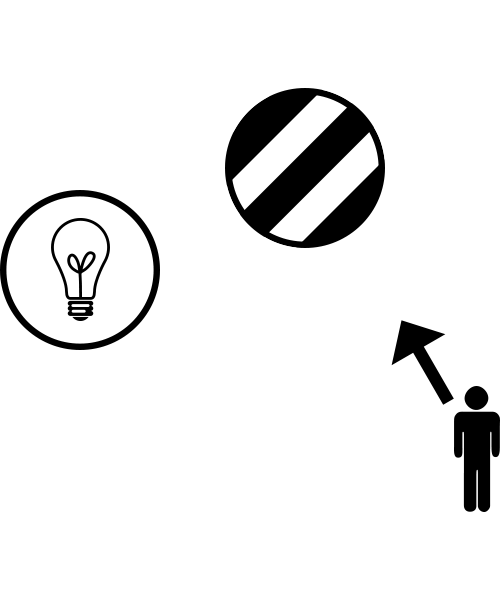
\includegraphics[height=5cm]{images/incorrect-positioning-estimate.png}
    \caption{Incorrect location estimate. The estimate is visualized as a striped circle.}
    \label{fig:indoor-positioning:incorrect}
\end{figure}

\begin{figure}[h]
    \centering
    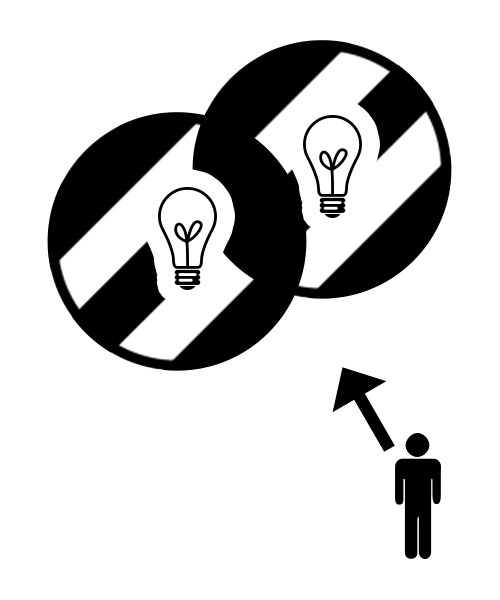
\includegraphics[height=5cm]{images/positioning-overlap.png}
    \caption{Overlap of estimated positions. The estimates are visualized as a striped circle.}
    \label{fig:indoor-positioning:overlap}
\end{figure}

Based on the above the following criteria for assessing potential solutions can be outlined.

\begin{itemize}
    \item Availability
    \item Price
    \item Ease of use
    \item Accuracy
\end{itemize}

Only solutions intended for indoor positioning was considered and thus GPS is not considered a potential solution. 
GPS is meant for outdoor positioning and a signal is not always available while indoors and even if it is, the accuracy of the estimated location is very low.

\begin{table}[h]
    \centering
    \caption{Assessment of potential solutions for indoor positioning. Please not that all prices are converted to U.S. dollars from their respective currency. Prices include the minimum available hardware for positioning a device.}
    \label{tbl:indoor-positioning}
    
    \begin{tabularx}{\textwidth}{XXXXX}
        \textbf{Product} & \textbf{Availability} & \textbf{Price} & \textbf{Ease of use} & \textbf{Accuracy} \\
        
        Estimote Beacons and Stickers \cite{estimote}
        & Beacons and Stickers are shipping. SDKs available.
        & \$99 for beacons. \$99 for 10 stickers, one per device to be positioned.
        & Initial installation of beacons. Attach each sticker to device.
        & Unknown. Desired to be less than five meters. \todo[author=Simon]{Update after conducting tests.} \\
        
        Pozyx \cite{pozyx}
        & Available for preorder.
        & \$368 for anchors. \$123 for each device to be positioned, plus supported Arduino.
        & Initial installation of anchors. One tag for each device, plus supported Arduino. Not meant for mounting.
        & Claimed to be 10 cm. Untested.
        
    \end{tabularx}
\end{table}

%%% Local Variables:
%%% mode: latex
%%% TeX-master: "../../master"
%%% End:
